\documentclass{article}

\usepackage{lmodern}
\usepackage[T1]{fontenc}
\usepackage[spanish,activeacute]{babel}
\usepackage{mathtools}
\usepackage{amsmath}
\usepackage[a5paper,margin=1in,top=15mm,bottom=15mm,landscape]{geometry} 
\usepackage{graphicx}

\title{\textbf{Pr\'actica 4}}
\author{\\Diego Jes\'us Romero Luque}
\date{\today}
\graphicspath{ {./images/} }

\begin{document}
\maketitle
\pagebreak
\begin{enumerate}
    \item Create the simplets WHILE programthat computes \textit{diverge} function 
        (with zero arguments) and compute the codification of its code.
        \begin{verbatim}
            octave:19> F("(1, X1:=X1+1; while X1!=0 do X1:=X1 od)", [0])
            complexity has reached 1000, press Ctrl-C to stop, or any other key to continue...
            
            octave:18> CODE2N("X1:=X1+1;while X1!=0 do X1:=X1 od")
            ans = 139126
        \end{verbatim}
    \pagebreak
    \item Create an Octave script that enumerates all the vectors
        \begin{verbatim}
            i = 0
            while (true)
                godeldecoding(i)
                i++
            endwhile
        \end{verbatim}
        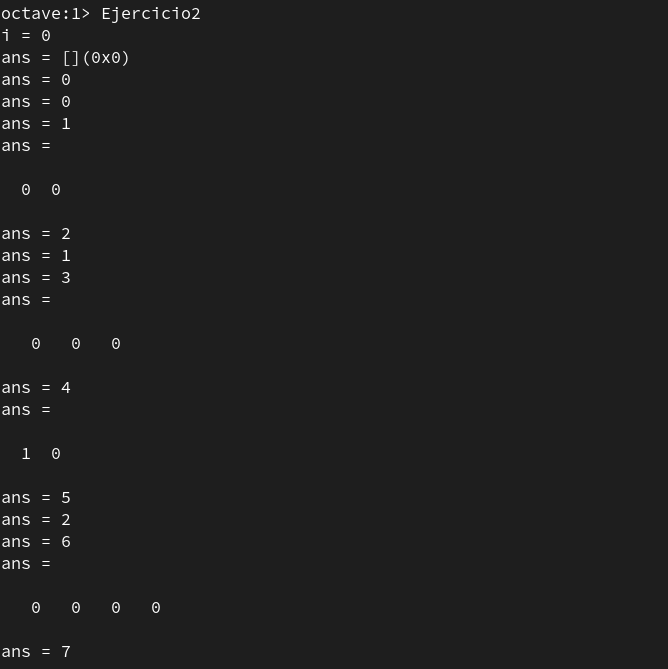
\includegraphics[scale=0.35]{Ej2.png}

    \item Create an Octave script that enumerates all the WHILE programs.
        \begin{verbatim}
            i = 0
            while (true)
                N2WHILE(i)
                i++
            endwhile
        \end{verbatim}
        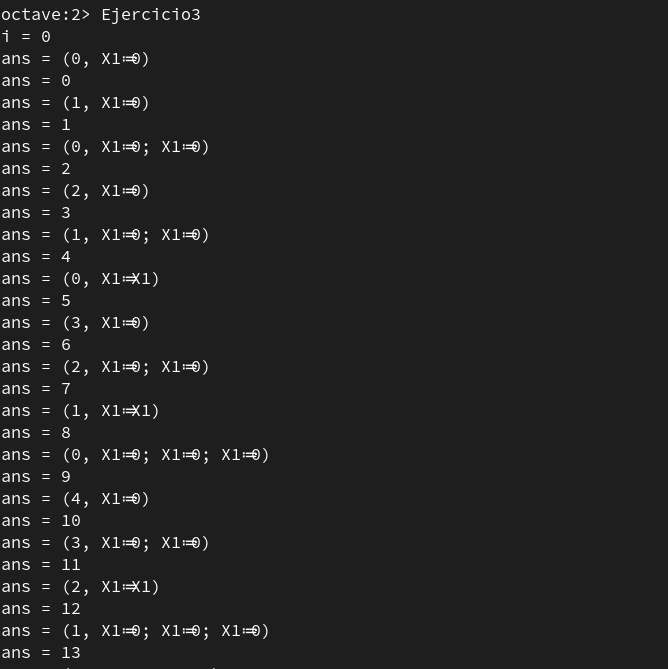
\includegraphics[scale=0.35]{Ej3.png}

    \end{enumerate}
\end{document}